%\documentclass{article}
%\usepackage[utf8]{inputenc}
%\title{test}
%\author{paolo.dini }
%\date{June 2017}
%\begin{document}
%\maketitle
%\section{Introduction}
%\end{document}

%===================================================
%================== DOCUMENT CLASS
%===================================================
\documentclass[runningheads,11pt,a4paper,english,llncs]{Misc/llncs}

%===================================================
%================== PACKAGES
%===================================================
%------------------------------------------------------------------------
% TeX and LaTeX macros
%------------------------------------------------------------------------
%
% In math formulas we use italic instead of mathitalic
%
\makeatletter
% ~ gives a \; space in math mode
\def~{\ifmmode\;\else\penalty\@M\ \fi}
%  Italic in mathematical formulas
\def\@setmcodes#1#2#3{{\count0=#1 \count1=#3
  \loop \global\mathcode\count0=\count1 \ifnum \count0<#2
  \advance\count0 by1 \advance\count1 by1 \repeat}}
\DeclareSymbolFont{italic}{OT1}{\rmdefault}{m}{it}
\let\mathit\undefined
\DeclareSymbolFontAlphabet{\mathit}{italic}
\edef\@tempa{\hexnumber@\symitalic}
\@setmcodes{`A}{`Z}{"7\@tempa41}
\@setmcodes{`a}{`z}{"7\@tempa61}
\makeatother
%
% \begin{asm} ... \end{asm}
%
\newdimen\asmindent     
\asmindent=\parindent
\newcount\asmi
\def\inc{\global\advance\asmi by 1}
\def\dec{\global\advance\asmi by-1}
\def\nl{{}$\par\hangindent\asmi em
  \noindent\kern\asmi em\ignorespaces$} 
\def\asmskip{{}$\par\smallskip\hangindent\asmi em
  \noindent\kern\asmi em\ignorespaces$} 
\def\asm{\global\asmi=0 
%%%%%%%%%%%%%% added by Paolo:
\parskip=0pt
%%%%%%%%%%%%%%%%%%%%%%%%%%%%%
 \def\+{\inc\nl}
 \def\-{\dec\nl}
 \def\\{\nl}
 \begin{trivlist}
 \item[]\leftskip=\asmindent\relax$}
\def\endasm{$
\end{trivlist}}
%\mathindent=\asmindent
%
% \begin{asmarray}
%    f(s_1) & := t_1 \\
%    f(s_2) & := t_2 
% \end{asmarray}
%
\def\asmarray{\begin{array}[t]{@{}l@{\;}l@{\;}l@{}}}
\def\endasmarray{\end{array}}
%
%
%
\def\asmcomment#1{\quad\hbox{// #1}}
%
%  \begin{subasm} ... \end{subasm}
%
\newcount\asmii
\def\subasm{\vtop\bgroup\asmii=0\normalbaselines
 \def\nl##1{$\egroup\advance\asmii by##1\relax\hbox\bgroup\hskip\asmii em$}
 \def\\{\nl{0}}
 \def\+{\nl{1}}
 \def\-{\nl{-1}}
 \hbox\bgroup\hskip\asmii em$}
\def\endsubasm{$\egroup\egroup}
%
% Keywords in ASM code
%
\def\ASM#1{\hbox{\sc#1}}        % rule names and macros
\def\ASMIND#1{\ASM{#1}\index{#1@{\sc#1}}}
\def\AWAIT   {\mathrel{\mathbf{await}}}
\def\AND     {\mathrel{\mathbf{and}}}
\def\CASE    {\mathrel{\mathbf{case}}}
\def\CHOOSE  {\mathrel{\mathbf{choose}}}
\def\CREATE  {\mathrel{\mathbf{create}}}
\def\NEW  {\mathrel{\mathbf{new}}}
\def\DO      {\mathrel{\mathbf{do}}}
\def\ELSE    {\mathrel{\mathbf{else}}}
\def\ELSEIF  {\mathrel{\mathbf{elseif}}}
\def\FORALL  {\mathrel{\mathbf{forall}}}
\def\FORSOME  {\mathrel{\mathbf{forsome}}}
\def\FOREACH  {\mathrel{\mathbf{foreach}}}
\def\IF      {\mathrel{\mathbf{if}}}
\def\IMPORT  {\mathrel{\mathbf{import}}}
\def\IN      {\mathrel{\mathbf{in}}}
\def\LET     {\mathrel{\mathbf{let}}}
\def\SELF    {\mathrel{\mathbf{self}}}
\def\MATCH    {\mathrel{\textbf{match}}}
\def\NOT     {\mathrel{\mathbf{not}}}
\def\OF      {\mathrel{\mathbf{of}}}
\def\OR      {\mathrel{\mathbf{or}}}
\def\PAR     {\mathrel{\mathbf{par}}}
\def\SEQ     {\mathrel{\mathbf{seq}}}
\def\SKIP    {\mathrel{\mathbf{skip}}}
\def\THEN    {\mathrel{\mathbf{then}}}
\def\WHERE   {\mathrel{\mathbf{where}}}
\def\WHILE   {\mathrel{\mathbf{while}}}
\def\UNDEF   {\mathrel{\mathbf{undef}}}
\def\UNTIL   {\mathrel{\mathbf{until}}}
\def\WHEN   {\mathrel{\mathbf{when}}}
\def\WITH    {\mathrel{\mathbf{with}}}
\def\STEP    {\mathrel{\mathbf{step}}}
\def\STEPWISE    {\mathrel{\mathbf{stepwise}}}
\def\SEQ    {\mathrel{\mathbf{seq}}}
\def\RESULT  {\mathrel{\mathbf{result}}}
\def\CALL  {\mathrel{\mathbf{Call}}}
\def\LOCAL    {\mathrel{\mathbf{local}}}
\def\ADDGUARD {\mathrel{\mathbf{addGuard}}}
\def\ADDUPD   {\mathrel{\mathbf{addUpd}}}
\def\ADDRULE  {\mathrel{\mathbf{addRule}}}
\def\MINUSRULE  {\mathrel{\mathbf{minusRule}}}
\def\TO      {\mathrel{\mathbf{to}}}
%
% Including figures
%
\def\includefig#1#2{\centering\medskip
  \includegraphics[scale=#1]{fig/#2}
  \medskip}
%
% References to paragraphs in the ECMA standard for C#
%
\def\ecma#1{\cite[\S#1]{ecma334}}
%
%  Environments for definitions and theorems
%
%\theorembodyfont{\rm}
%\newtheorem{definition}[subsection]{Definition}
%\newtheorem{lemma}[subsection]{Lemma}
%\newtheorem{theorem}[subsection]{Theorem}
%\newtheorem{proposition}[subsection]{Proposition}
%\newtheorem{corollary}[subsection]{Corollary}
%\newtheorem{example}[subsection]{Example}
%\newtheorem{remark}[subsection]{Remark}
%\newtheorem{constraint}[subsection]{Constraint}
\def\proof{\trivlist\item[]{\bf Proof.}}
\def\endproof{$\Box$\endtrivlist}
%
% enumerate and itemize (smaller skips) from "latex.ltx"
%
\makeatletter
\def\enumerate{%
  \ifnum \@enumdepth >\thr@@\@toodeep\else
    \advance\@enumdepth\@ne
    \edef\@enumctr{enum\romannumeral\the\@enumdepth}%
      \expandafter
      \list
        \csname label\@enumctr\endcsname
        {\usecounter\@enumctr\def\makelabel##1{\hss\llap{##1}}
         \itemsep 0pt\parskip 0pt\parsep 0pt\topsep\smallskipamount}%
  \fi}
\def\itemize{%
  \ifnum \@itemdepth >\thr@@\@toodeep\else
    \advance\@itemdepth\@ne
    \edef\@itemitem{labelitem\romannumeral\the\@itemdepth}%
    \expandafter
    \list
      \csname\@itemitem\endcsname
      {\def\makelabel##1{\hss\llap{##1}}
       \itemsep 0pt\parskip 0pt\parsep 0pt\topsep\smallskipamount}%
  \fi}
\makeatother
%
% items in itemize
%
\def\bull{\vrule height .9ex width .8ex depth -.1ex}
\def\labelitemi{\bull}
%
%
%
\def\cs#1{C\#$_{\mathcal{#1}}$}
\def\lang#1{L$_{\mathcal{#1}}$}
%
% Positions
%
\def\pos#1{{}^{#1}}
\def\termPos{\blacktriangleright}
\def\cursor{\pos{\termPos}}
%
%
%
\def\sup{\hbox{sup}}
\def\c#1{\texttt{#1}}           % code
\def\N#1{\textit{#1}}           % non terminal symbols
\def\T#1{\hbox{`\texttt{#1}'}}  % terminal symbols
\def\A#1{\hbox{\sc#1}}          % ASM rules
\def\D#1{#1}                    % dynamic functions
\def\U#1{#1}                    % universes
\def\C#1{#1}                    % constructors
\def\rdef{\equiv}
\def\lbr{\c{\char`\{}}
\def\rbr{\c{\char`\}}}
\def\mb{\hbox{::}}
\def\map#1#2{\textbf{Map from}~#1~\textbf{to}~#2}
\def\cat{\cdot}
\def\adots{\mathinner{\ldotp\ldotp}}
%
%
% macros.tex ends here

\usepackage{etex}
\reserveinserts{28}
\newcommand{\todo}[1]{
 \noindent{\newline \color{red}
 \framebox[\textwidth][t]{%
  \parbox[t]{0.9\textwidth}{\textcolor{red}{TODO: #1}}                                                                                     
}}}


%===================================================
%================== PACKAGES
%===================================================
\usepackage{graphicx}
\usepackage{acronym}
\usepackage{ifthen}
\usepackage{substr}
\usepackage{color}
\usepackage{fixltx2e}
\usepackage[left=2cm, top=2cm, right=2cm, bottom=2cm]{geometry}
%\usepackage{subfigure}
\usepackage{array,rotating}          
\usepackage{url}
%\usepackage{enumerate}
\usepackage[shortlabels]{enumitem}
\usepackage{epsfig}
\usepackage{colordvi}
\usepackage{makeidx}
\usepackage{index}
\usepackage[absolute]{textpos}
\setlength{\TPHorizModule}{\paperwidth}
\setlength{\TPVertModule}{\TPHorizModule}
\textblockorigin{-6mm}{0mm}
\usepackage[%
      breaklinks=true,%
      colorlinks=true,%           no frame around URL
      urlcolor=LINK_COLOR,%            no colors
      menucolor=LINK_COLOR,%           no colors
      linkcolor=LINK_COLOR,%           no colors
      pagecolor=LINK_COLOR,%           no colors
      bookmarks=true,%            tree-like TOC
      bookmarksopen=false,%       expanded when starting
      hyperfootnotes=true,%       no referencing of footnotes, does not compile
      citecolor=CITE_COLOR,%           black cites
      filecolor=black,%           black files%
      hyperindex=true,%
      hyperfigures=true%
]{hyperref}
\usepackage{bookmark}
\usepackage{dsfont}
\usepackage{wallpaper}
\usepackage{mathtools,cancel}
\usepackage{soul}
\usepackage{float}
\usepackage{setspace}
%\usepackage{morefloats}
%\usepackage{mdwlist}
\usepackage{amsmath,amssymb,amscd,diagrams,bm,amsfonts}
\let\proof\relax
\let\endproof\relax
\usepackage{amsthm}
\usepackage{tabularx, graphics, longtable}
%TIKZ
\usepackage{tikz}
\usepackage{tikz-cd}
\usetikzlibrary{trees,snakes}
\usetikzlibrary{arrows,automata}
\usetikzlibrary{matrix,arrows,positioning}
\usetikzlibrary{mindmap,backgrounds}
\usetikzlibrary{shapes}
\usepackage{verbatim} %for comment out some texts


%%%%%%%%%%%%%%%%%%%%%%%%%%%%%%%
%%%%%%%%%%%%%%%%%%%%% Egon's commands:
\usepackage{latexsym}
\ifx\pdfoutput\undefined
  \message{We are running LaTeX.} 
%PD  \usepackage[dvips]{graphicx}
%PD  \DeclareGraphicsExtensions{.eps}
%PD  \usepackage[hypertex,bookmarks=false]{hyperref}
\else
  \message{We are running PDFLaTeX.}
%PD  \usepackage[pdftex]{color}
%PD  \usepackage[pdftex]{graphicx}
%PD\DeclareGraphicsExtensions{.jpg,.pdf}
%PD  \DeclareGraphicsExtensions{.pdf}
%PD  \usepackage[pdftex,bookmarks=false]{hyperref}
%PD  \hypersetup{colorlinks={true},
%PD            linkcolor={blue},
%PD            citecolor={blue},
%PD            urlcolor={blue},
%PD            plainpages={false}
%PD  }
\fi
%%%%%%%%%%%%%%%%%%%%%%%%%%%%%%%
%%%%%%%%%%%%%%%%%%%%%%%%%%%%%%%


%===================================================
%================== COLOURS
%==================================================

\definecolor{green}{rgb}{0,0.6,0} 
\definecolor{gray}{rgb}{0.6,0.6,0.6} 
\definecolor{red}{rgb}{1,0,0} 
\definecolor{blue}{rgb}{0,0,1} 
\definecolor{purple}{rgb}{0.5,0,0.5} 
\definecolor{yellow}{rgb}{0.25,0.25,0} 
\definecolor{turquoise}{rgb}{0,0.5,0.5}
\definecolor{brown}{rgb}{0.6,0.2,0.1}

\definecolor{LINK_COLOR}{rgb}{0,0,0.7}
\definecolor{CITE_COLOR}{rgb}{0,0.5,0}
\definecolor{lightblue}{rgb}{0,0,1}
\definecolor{light-gray}{gray}{0.95}
\def\red#1{\textcolor[rgb]{1.0,0.0,0.0}{#1}}
\def\green#1{\textcolor[rgb]{0.0,0.8,0.1}{#1}}
\def\blue#1{\textcolor[rgb]{0.0,0.0,1.0}{#1}}

%===================================================
%================== LAYOUT
%===================================================
\parindent=0cm
%\setlength{\parskip}{1.0\baselineskip plus 0.5ex minus 0.2ex}
\abovecaptionskip=0cm
\hyphenpenalty=5000
\tolerance=1000 
\floatsep=1in
\allowdisplaybreaks
\def \constzeroindent {0cm}
\def \constfirstindent {0.5cm}
\def \constsecondindent {1cm}
\newenvironment{mycustomindent}[1]
{\setlength{\parindent}{#1}}
{\setlength{\parindent}{\constzeroindent}}
\newcommand{
	\firstindent}[1]{
	\begin{mycustomindent}{\constfirstindent}
	\begin{tabular}{@{}p{12cm}@{}}
	#1 \\
	\end{tabular}
	\end{mycustomindent}
}
\newcommand{
	\secondindent}[1]{
	\begin{mycustomindent}{\constsecondindent}
	\begin{tabular}{@{}p{12cm}@{}}
	#1 \\
	\end{tabular}
	\end{mycustomindent}
}
\newenvironment{packed_item1}{
\begin{itemize}[topsep=0pt, partopsep=0pt]
  \setlength{\itemsep}{5pt}
  \setlength{\parskip}{0pt}
  \setlength{\parsep}{0pt}
}{\end{itemize}}
\newenvironment{packed_item2}{
\begin{itemize}[topsep=0pt, partopsep=0pt]
  \setlength{\itemsep}{0pt}
  \setlength{\parskip}{0pt}
  \setlength{\parsep}{0pt}
}{\end{itemize}}
\newenvironment{packed_enumerate}{
\begin{enumerate}[topsep=0pt, partopsep=0pt]
  \setlength{\itemsep}{5pt}
  \setlength{\parskip}{0pt}
  \setlength{\parsep}{0pt}
}{\end{enumerate}}
% The following commands are to get rid of the extra space around section and subsection titles:
% Save the class definition of \subparagraph:
\let\llncssubparagraph\subparagraph
% Provide a definition to \subparagraph to keep titlesec happy:
\let\subparagraph\paragraph
\usepackage[compact]{titlesec}
\usepackage{dblfloatfix,caption,subcaption}
\titlespacing{\section}{0pt}{12pt}{*0}
\titlespacing{\subsection}{0pt}{6pt}{0pt}
\titlespacing{\subsubsection}{0pt}{6pt}{0pt}
% Force section numbering to follow chapter numbering:
\usepackage{chngcntr}
\counterwithin{section}{chapter}
\counterwithin{figure}{chapter}
%\counterwithin{theorem}{chapter}
%\counterwithin{lemma}{chapter}
%\counterwithin{definition}{chapter}
%%%%%%%%%%%%%%%%%%%%%%%%%%%%
% Allow line breaks in long list of citations that would extend into the margin:
\usepackage{breakcites}
%%%%%%%%%%%%%%%%%%%%%%%%%%%%%%%%%%%%%%

\usepackage{pdfpages}
\pagestyle{headings}

\renewcommand{\rightmark}{INTERLACE Project (Grant no.~754494)}
\renewcommand{\leftmark}{D2.1}
\setcounter{tocdepth}{2}

\usepackage{tocloft}
\setlength\cftparskip{0pt}
\setlength\cftbeforechapskip{12pt}

\usepackage{abstract}
\renewcommand{\abstractnamefont}{\large \bfseries}
%\setlength{\abstitleskip}{-\absparindent}
\renewcommand{\abstractname}{Abstract}

\setlength{\parskip}{12pt}

\begin{document}
%===================================================
%================== TITLE
%===================================================

\thispagestyle{empty}
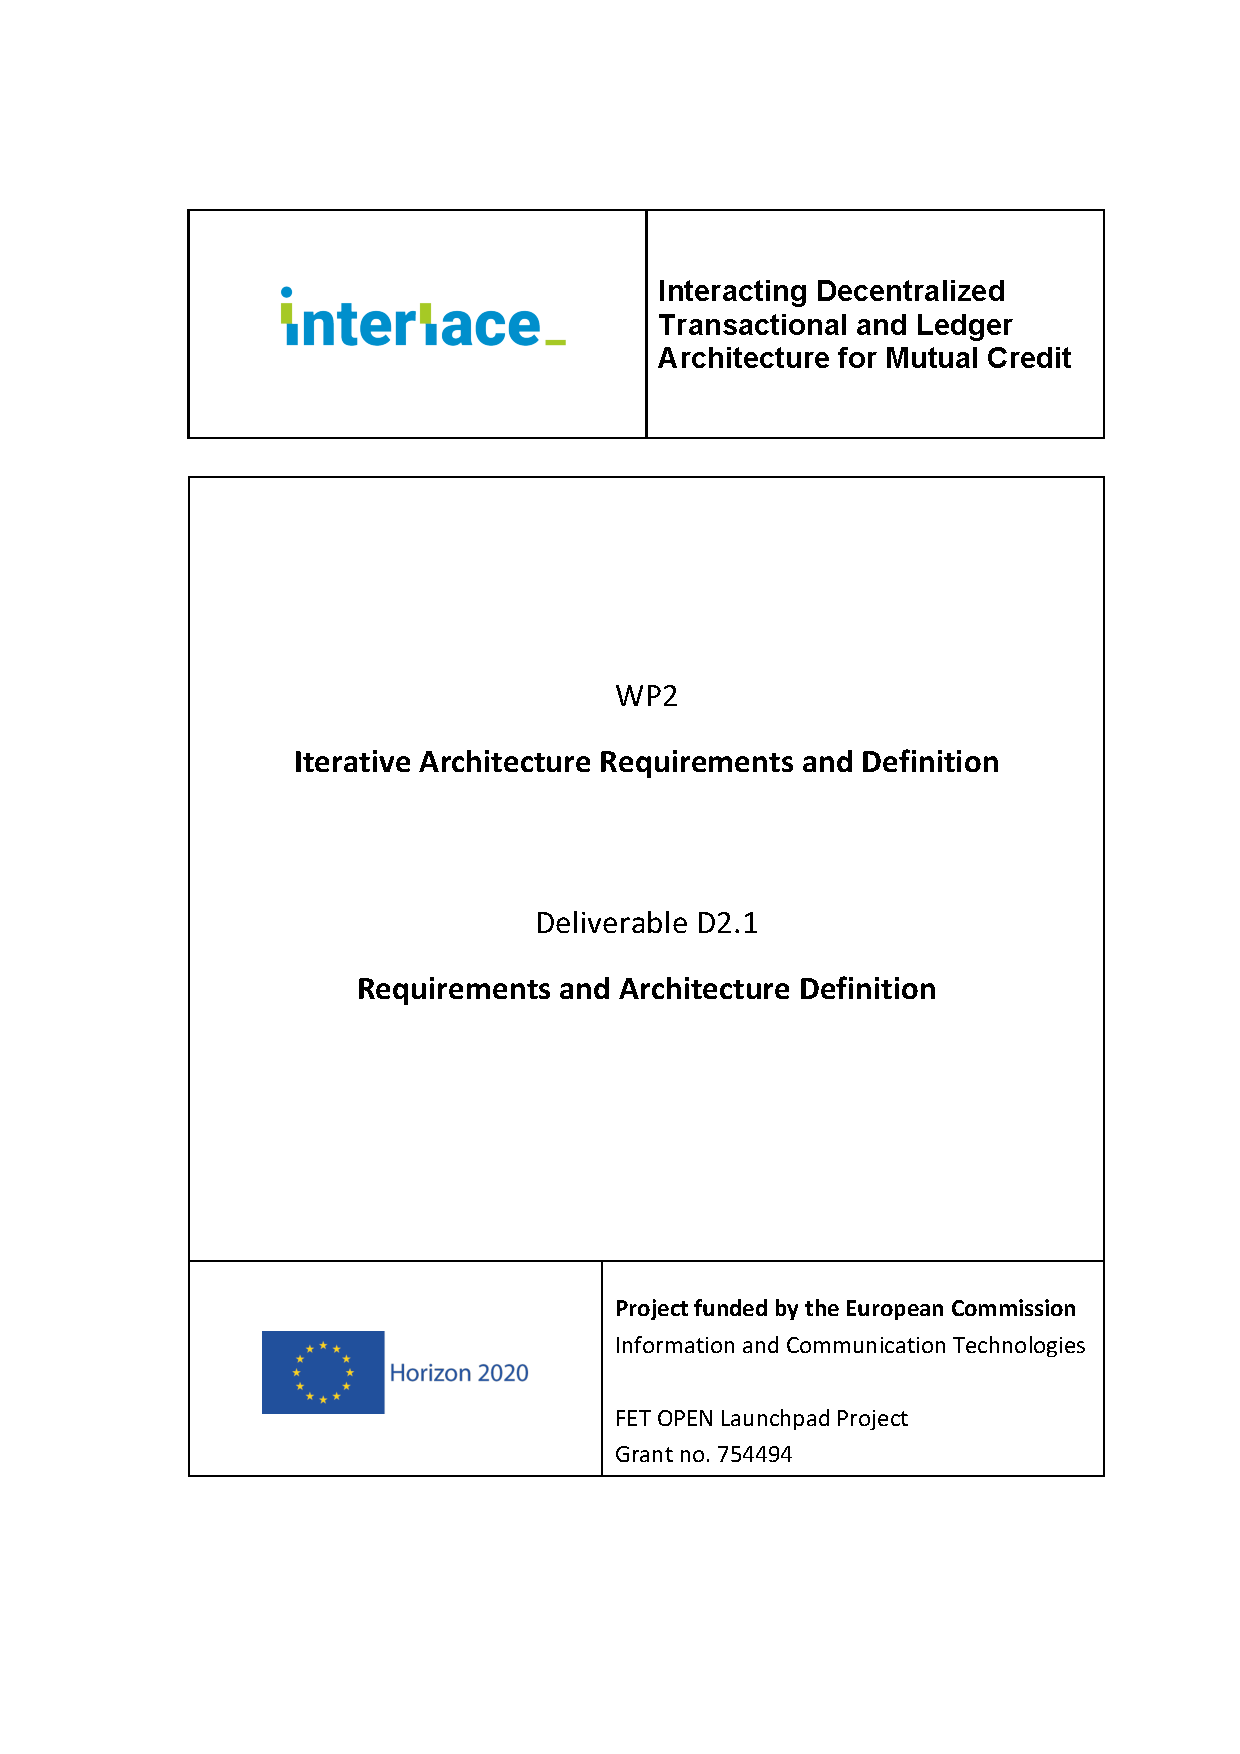
\includepdf[pages=-, scale=1.0]{Misc/Front}

%===================================================
%================== ABSTRACT
%===================================================
\thispagestyle{empty}

\begin{abstract}
\normalsize



\end{abstract}

\newpage

%===================================================
%================== TABLE OF CONTENTS
%===================================================
\tableofcontents

%===================================================
%================== CHAPTERS
%===================================================
\chapter{Introduction}
\label{ch:Introduction}

\vspace{-1cm}
\begin{center}
Paolo Dini and Giuseppe Littera
\end{center}

The INTERLACE project is developing a blockchain-based transactional platform for use by the Sardex mutual credit system. Sardex S.p.A. (SARDEX) has been operating successfully an electronic, B2B, zero-interest mutual credit system on the island of Sardinia since 2009. The Sardex system (also known as Circuito di Credito Commerciale) challenges prevailing notions about the nature of money, and the financial and economic autonomy that a relatively poor region can aspire to, because it enables local economic actors (SMEs in particular) to trade with each other in a trustful and circular fashion with a unique digital trade credit unit. It does this by monetizing the spare capacity of the local economy in the form of mutual, and taxable, credit between participating companies, at zero interest, on a strong basis of trust, solidarity, and local cultural identity \cite{LitteraEtAl2017,DiniMottaSartori2016,SartoriDini2016}. The deeply innovative nature of this system is to distribute to the circuit members the power to create credit money (sardex credits, where 1 credit = 1 Euro), and thereby provide an alternative to credit money creation through bank loans. However, the Sardex transactional platform is currently centralized,\footnote{Cyclos 4: \url{http://www.cyclos.org/products/}.} which challenges the long-term scalability, sustainability, and governance of the system because the governance and management of the circuit are all held by the central credit-clearing entity (SARDEX).

The specification and implementation of the new architecture is based on the Abstract State Interaction Machines (ASIMs), developed and implemented in the platform CoreASIM by the BIOMICS project\footnote{\url{http://biomicsproject.eu/}} \cite{BIOMICSD41,BIOMICSD42,BIOMICSD52} as extensions of B\"orger and St\"ark's \cite{BoergerStaerk2003} Abstract State Machines (ASMs) and of the CoreASM environment.\footnote{\url{http://biomicsproject.eu/news/135-icef}} The ASIMs are based on realizing the BIOMICS mathematical framework for Interaction Machines (IMs) that dynamically and recursively grow and change their components and network topologies to deploy/reabsorb resources in response to interactions and computational needs \cite{NehanivEtAl2015}. Relative to the ASMs, ASIMs are fully asynchronous, concurrent, and communicating, so they can run on different servers and communicate over the network to validate transactions. The ASIM approach is fundamentally important for SARDEX as a company because it guarantees verifiability, validation, and efficient change management (to manage requirements creep as well as new emerging functionalities) through rigorous mathematical formalization of the specification at the level of requirements capture and a rigorous process of iterative refinement down to the level of the code of choice. Any of these levels of abstraction is executable by an interpreter (built into coreASIM), so at each level of the refinement process the current implementation level can be verified against requirements.

The number of new cryptocurrencies is increasing very rapidly,\footnote{As of 28/08/17 there were 865 currencies listed on \url{https://coinmarketcap.com/}, up from 851 a few days earlier.} along with the variations in the technologies that support them. This very volatile technology landscape is causing us to focus first on the new economic and governance model for sardex.net, which will provide the high-level requirements for the new blockchain architecture and will, therefore, enable us to narrow down the number of possible frameworks and technologies to draw from. In the meantime, we have begun the non-trivial task of migrating the current platform functionality towards the new model. The first step in this process has been to begin formalizing the SARDEX business logic as ASM models.

This report is organized as follows. Chapter \ref{ch:archreq} provides a high-level view of the architecture and its documentation following the arc42 method.\footnote{\url{http://arc42.org/}} Chapter \ref{ch:funreq} provides a first collection of functional requirements of the system modelled as ASMs. These reflect the business logic of the \emph{current} system. This model will be instantiated in CoreASIM in order to execute it with a fictitious set of inputs and verify its operation, after which it will be implemented in a language of choice (probably Java).

A second specification and modelling effort will follow, to reflect in the blockchain ``backend'' the new governance and financial/economic model once it has been completed. This second model and its implementation will be reported in the next architecture deliverable (D2.2) at Month 12.












\chapter{Modelling Sardex Payment Operations\\ (Functional Requirements)}
\label{ch:funreq}


\vspace{-1cm}
\begin{center}
Egon B\"orger
%, Luca Carboni, Massimeddu Cireddu, Paolo Dini, Eduard Hirsch
\end{center}


We specify the core payment and related history operations of the Sardex system. We do this at the functional requirements  level of abstraction and in a component-based manner so that the resulting model can serve as abstract description of the current implementation but also as starting point for a new, blockchain-based implementation. Sect.~\ref{sect:paymtops} models  two basic payment operations, Sect.~\ref{sect:accHistory} account history and balance operations, Sect.~\ref{sect:permission} permission features, Sect.~\ref{onboarding} onboarding operations and Sect.~\ref{sect:userops} user operations.


\section{Core Payment Operations}
\label{sect:paymtops}

In this section we describe the interaction of the Sardex system (also called simply Sardex)  with users. We consider here B2B operations, leaving the consideration of operations between a company and either employees or consumers for a later phase. Sect.~\ref{signaturepaymtop} explains the basic data types,  Sect.~\ref{sec:creditop} the credit and  Sect.~\ref{sec:debitop} the debit operation.

\subsection{Signature elements of B2B Operations}
\label{signaturepaymtop}
The actors of B2B operations are companies which interact with the Sardex system on a request/response basis using various 
communication devices from whose technical details we abstract here. Therefore it comes natural to describe the interaction of companies with the Sardex system by $\ASM{Send}$ and $\ASM{Receive}$ actions of communicating Abstract State Machines (ASMs), the basic concept underlying Abstract State Interaction Machines (ASIMs)\footnote{ASIMs are communicating ASMs which are equipped with a general scheduling mechanism and an interaction structure to distinguish
between horizontal and hierarchical interaction. These features have
been defined to satisfy the requirements of Interaction Computing
formulated in Deliverable 5.1 of the BIOMICS project  \cite{BIOMICSD51}; these requirements have been shown to be satisfied by ASIMs (see Ch.\ 2 of
Deliverable D5.2 \cite{BIOMICSD52}). For further details (in particular on the
definition of the communication network structure, using channels and
a routing component, and a resource manager by specialized
communicating ASMs) and the implementation see
\url{https://github.com/biomics/icef}.}, one for each participating company and one for Sardex.\footnote{Observe that in a distributed version of the Sardex system different instances of the system are run by different agents which all execute the same ASM program (or a program that has been obtained by adapting the basic program appropriately for a particular instance). Cyclos today is monolithic. \textcolor{green}{It can be distributed because you can have multiple applications running on multiple machines that share consistency with third-party utilities. So, we can use the term modular or simply  ``loosely coupled''.}} We concentrate our attention in this section on modelling the actions the Sardex system performs when triggered by requests sent to it by any company of the circuit (which are treated in Sec.~\ref{sect:userops}).

We keep the communication mechanism abstract. $\ASM{Send}(msg,to(a))$ denotes the operation of sending the $msg$ to agent $a$. 
$Received(msg,from(s))$ is a predicate which is true when the message $msg$ from the sender $s$ is in the $mailbox$ of the receiver. $\ASM{Consume}(msg)$ denotes the operation of deleting the $msg$ from the $mailbox$ once it is processed. 

We usually assume  each $msg \in Message$ to contain besides its $payload(msg)$ also the information about its $sender(msg)$ and $receiver(msg)$. Thus the parameter $from(c)$ in $Received(msg, from(c))$ indicates that $sender(msg)=c$. Similarly, $to(c)$ in $\ASM{Send}(msg, to(c))$ denotes that $receiver(msg) = c$.

The core payment operations are sent to Sardex by companies $c \in SardexNet$ which are members of the net.\footnote{We use for the datatypes evocative names which suggest their intended interpretation.} \textcolor{purple}{(Massi) A company can has at most an account for each account type.} Each such company may have a number of $acc$ounts which we represent as elements of a set $Account(c)$. Each $acc$ount has a well-defined $owner(acc) \in SardexNet$ and is of some type $accountType(acc)$ out of the set $AccountType$ of possible account types:

\begin{asm}
AccountType=\{credit, domu, fee\} \\
Account = \bigcup_{c \in SardexNet} Account(c)
\end{asm}
Therefore we name such accounts $creditAccount(c)$, $domuAccount(c)$, $feeAccount(c)$ (names which are defined if $c$ has the corresponding accounts). 

There are two principal transfer operations, called Credit and Debit operation specified in Sect.~\ref{sec:creditop} and Sect.~\ref{sec:debitop}.

\subsection{Sardex Behaviour for Credit Operations}
\label{sec:creditop}

A Credit operation is also called a push transfer. Its goal is to transfer an $amount$ via a specific $channel$ from one account to another. Sardex uses a $TransferType$ concept which allows one to impose on the transfer operations certain conditions, including priorities. The parameters of a transfer type $tt$ which are relevant for the Sardex business logic are the following:\footnote{The implementation in Cyclos has more parameters we do not consider here.}

\begin{itemize}
	\item the $operation \in \{credit, debit\}$,
	\item the $channel \in \{phone,website,pos\}$\footnote{$pos$ abbreviates point of sale.} through which the interaction between the user and Sardex takes place,
	\item the account type of the two involved accounts $from,to \in Account$,
	\item \textcolor{purple}{(Massi) the groups of the two members involved: $fromMemberGroup,toMemberGroup \in Group$ }
	\item conditions on the to-be-transferred $amount$, 
	\item conditions on so-called custom fields.
\end{itemize}

The $custFieldCond$ition may be empty (formally speaking defined as True, i.e. always satisfied). We retrieve for each parameter the corresponding information from a transfer type $tt$ by an appropriate function:

\begin{asm}
name\colon TransferType \rightarrow Identifier \\
oper\colon TransferType \rightarrow Operation\\
chan\colon TransferType \rightarrow Channel \\
sourceType,destType\colon TransferType \rightarrow Formula 
       \mbox{ // expressions for conditions}\\
amountCond,custFieldCond\colon TransferType \rightarrow Formula\\
\WHERE \+
    Operation = \{credit,debit\} \\
    Channel = \{phone, website,pos\}
\end{asm} 

One can imagine $TransferType$ as a table where each row is named and contains the parameters of the represented $tt$. The $TransferType$ data type is defined in such a way as to guarantee the following property: 
\begin{quote} 
	{\bf Transfer Type Welldefinedness}. For each transfer $operation \in \{credit,debit\}$ and each pair of accounts $acc,acc'$ there is at most one $tt \in TransferType$, i.e. at most one $tt$ which satisfies
	\begin{itemize}
		\item $oper(tt) = operation$,
		\item $sourceType(tt)=accountType(acc)$,
		\item $destType(tt)=accountType(acc')$.
	\end{itemize} 
We denote this unique $tt$ as the value of the function $tt(operation,acc,acc')$.\footnote{Following common notation we use the same name $tt$ for elements of $TransferTable$ and for the function $tt(params)$; it will always be clear from the context which one is meant.}
\end{quote}

\vspace{12pt}
\textcolor{red}{***QUESTION 1 to Luca/Massi: This implies that given any $operation$ and two accounts $acc,acc'$, the channel through which the operation is allowed to be performed is unique, defined by the unique $tt \in TransferTable$ for $operation,acc,acc'$. Why is this required? ***}
\vspace{12pt}

Both payment operations Credit and Debit are instances of a request/response pattern with two phases, a first phase whose action is called Preview -- where only the permission for the transfer is checked (using a $transferTypeCheck$ function) but not the requested amount -- and  a second phase whose action is called Perform where also the amount is checked (using a $balanceCheck$ function). On the user side both actions are treated as stateless, on the Sardex system side only the Preview action is stateless. 

Various notations are available to make the sequential character of two successive steps explicit in the context of the parallel computation model of ASMs. One is to use a traditional flowchart definition (which visualizes the explicit introduction of successive $mode$ or $phase$ values and ends up defining what are called control-state ASMs). Another one is to use the $\STEP$ operator for ASMs which is defined in such a way that in two successive executions of $M \STEP N$, in the first step $M$ and in the second step $N$ is executed, in the next execution of  $M \STEP N $ again $M$, etc. Here we make the -- for the user stateless -- two-phase interaction explicit by using two  types of user requests, say $CreditPreviewReq$ and $CreditPerformReq$, assuming that the user first sends a $CreditPreviewReq$uest and upon the positive system response the corresponding $CreditPerformReq$uest. Since Sardex when responding to a $CreditPreviewReq$uest does not record the data (due to the requirement of the stateless Preview response character), when elaborating a $CreditPerformReq$uest the system in a first step must redo the $transferTypeCheck$. 

The function $availBalance(acc)$ yields the amount of money that is currently available in the $acc$ to be spent. It is defined together with the related current balance function $balance(acc)$ in Sect.~\ref{sect:accHistory}. $Receivable(amount,acc)$ checks whether the destination of the transfer by receiving the $amount$ would exceed its upper Sardex limit $upperLimit(acc)$.

To illustrate a high-level specification of error cases we define the function $balanceCheck$ to yield \textcolor{brown}{a set which contains either the information that the condition to be checked is true or the set of causes which violate the condition $<<$--- NOT CLEAR}. Out of this set an $ErrMsg$ can be constructed to provide the user with some information why the $balanceCheck$ did not succeed (if any). 

\begin{asm}
\ASM{CreditTransferReq}(( channel,from, to, amount),mbr)=\+
\LET transfer=(credit,channel,from,to,amount) \\
\IF  Received(CreditPreviewReq(transfer),from(mbr)) \THEN \+  
   \LET res=transferTypeCheck(transfer)  \+
      \IF res = transferTypeError(transfer) \THEN \+ \ASM{Send}(ErrMsg(NotPermitted(transfer,res)),to(mbr))\-
      \IF res=ok \THEN ~ \ASM{Send}(YouMayProceedWith(transfer),to(mbr))\dec\-
\IF Received(CreditPerformReq(transfer),from(mbr)) \THEN \+     
    \LET res=transferTypeCheck(transfer)  \+
       \IF res = transferTypeError(transfer) \THEN \+ \ASM{Send}(ErrMsg(NotPermitted(transfer,res)),to(mbr))\+
          \ELSE~ \LET bal = balanceCheck(from, to, amount) \+
              \IF bal=ok \THEN ~ \ASM{Append}(transaction(transfer),Ledger)\+
                \ELSE ~ \ASM{Send}(ErrMsg(transfer,bal),to(mbr))\dec\dec\dec\dec\dec\-
\WHERE \+
  transferTypeCheck(transfer)=\+
           \left\{\begin{array}{ll}
           ok & \IF ~ \FORSOME tt \in TransactionType ~~  Match(tt,transfer)\\
           transferTypeError(transfer) & \ELSE 
           \end{array}\right .\-
  \LET transfer=(credit,channel,from,to,amount) \+
       Match(tt,transfer) \mbox{ if } \+
          oper(tt)=credit \AND chan(tt)=channel \AND \\
          sourceType(tt)=accountType(from) \AND destType(tt)=accountType(to) \AND \\
              custFieldCond(tt)(??)=true\dec\-
  info \in balanceCheck(from, to, amount)  \IFF \+
     info= ok  \AND amountCond(tt(credit,from,to))(amount) =true \AND \+
         availBalance(from) \geq amount \AND Receivable(amount,to)\-
     info = ViolatesAmountCond(amount) \AND \+
               amountCond(tt(credit,from,to))(amount) = false \-
     info=ViolatesLowerLimit(from,amount) \AND availBalance(from) < amount \\
     info=ViolatesUpperLimit(to,amount) \AND  ~\NOT Receivable(amount,to) \-
 Receivable(amt,acc) \mbox{ iff } balance(acc) + amt \leq upperLimit(acc)
\end{asm}

\vspace{12pt}
\textcolor{red}{***QUESTION 2 to Luca/Massi: Should the customfield information be included as one of the $transfer$ parameters? I guess the $custFieldCond(tt)$ is checked by the transfer type check, or not?***}
\vspace{12pt}

The $Match$ predicate is extended in Sect.~\ref{sec:debitop} for $debit$ transfer parameters.

The function $transaction(transfer)$ denotes the final transaction corresponding to the given $transfer$. It depends on the concrete $transfer$ data $(credit,channel,from,to,amount)$ (which must $Match$ some transfer type) but provides also other information, e.g. the $date$ of the transfer, the used transfer type, etc.

\vspace{12pt}
\textcolor{red}{***QUESTION 3 to Luca/Massi: Should such additional parameters be included
	into the arguments of the $transaction(transfer)$ function? In that case: what is the set of these parameters (explained conceptually, leaving their exact data type description to a refinement step)?***}
\vspace{12pt}

In the $\ASM{CreditTransferReq}$ model we assume that its access to the two accounts $from, to$ is exclusive; in other words, we abstract here from the corresponding synchronization mechanism which guarantees the assumption.

The error reporting function $transferTypeError(transfer)$ can be defined by distinguishing the cases one wants to consider. This allows one to tailor accordingly the format and payload of the function  $ErrMsg$ which constructs error messages. For the sake of illustration we provide here a possible definition for  $transferTypeError(transfer)$ (which is computed as part of the computation of $transferTypeCheck(transfer)$).

\begin{asm}
\LET transfer=(credit,channel,from,to,amount) \\
transferTypeError(transfer)=\+
  \mbox{No $credit$ opn is allowed from an account of $accountType(from)$}\\ 
  \OR \mbox{You are note allowed to use this $channel$ for a $credit$ opn}\\
  \OR \mbox{No $credit$ opn is allowed to an account of $accountType(to)$}\\
    \OR \ldots ???
\end{asm}
\vspace{12pt}
\textcolor{red}{***QUESTION 4 to Luca/Massi: Which are the error cases you would like to be dealt with here?***}
\vspace{12pt}


\subsection{Sardex Behaviour for Debit Operations}
\label{sec:debitop}

Similarly to Credit operations, also for a Debit operation between two network members $creditor,debitor$ Sardex accepts a $DebitPreviewReq$uest and a  $DebitPerformReq$uest from a $creditor$, using two corresponding rules $\ASM{DebitPreviewReq}$ and $\ASM{DebitPerformReq}$.  $DebitPerformReq$uests are executed using a request/response interaction between the system and the $debitor$. The $debitor$ has to allow the transfer by acknowledging a $ConfirmationReq$uest Sardex sends out; only when the debit transfer has been permitted by an acknowledgement from the $debitor$ will Sardex execute the transfer using a third rule called $\ASM{DebitAckExec}$ution. 

Sardex can execute at any moment any of these rules whose execution depends only on the parameters with which they are called. But for one successful debit $request$ instance the three rules can be executed only in the indicated order, due to the intrinsic sequentiality of the three steps for the $request$.

\begin{asm}
\ASM{DebitTransferReq}=\+
   \ASM{DebitPreviewReq} \\
   \ASM{DebitPerformReq} \\
   \ASM{DebitAckExec}
\end{asm}


Both rules $\ASM{DebitPreviewReq}$ and $\ASM{DebitPerformReq}$ in their first step make a $transferTypeCheck$ for the account of type $credit$ of the $debitor$, defined by extending the $Match$ predicate for $debit$ transfer operations. 

\begin{asm}
\ASM{DebitPreviewReq}((debitor,amount,channel),creditor)=\+
  \IF Received(DebitPreviewReq(debitor,amount,channel),from(creditor)) \THEN \+  
    \LET from=creditAccount(creditor), to=creditAccount(debitor)\\
    \LET transfer=(debit,channel,from,to,amount), res=transferTypeCheck(transfer) \+
        \IF res = transferTypeError(transfer) \THEN \+                       \ASM{Send}(ErrMsg(NotPermitted(transfer,res)),to(creditor))\-
        \ELSE~ \ASM{Send}(YouMayProceedWith(transfer),to(creditor))\dec\-
\WHERE \+
  Match(tt,transfer) \mbox{ if } \+
        oper(tt)=debit \AND chan(tt)=channel \AND \\
        sourceType(tt)=accountType(from) \AND destType(tt) =  accountType(to) \AND \\ custFieldCond(tt)(????)=true
\end{asm}

\vspace{12pt}
\textcolor{red}{***Question 5 to Luca/Massi:  Is this $Match$ definition for $debit$ correct or should the account parameters be inverted so that a $debit$ $Match$ holds if the $credit$ $Match$ holds on the accounts with inverted order?***}
\vspace{12pt}

If the $transferTypeCheck$ in a $ \ASM{DebitPerformReq}$uest succeeds, a two-phase request/response interaction is started, this time with the system as requestor to which the $debitor$ responds. More precisely upon receiving the $DebitPerformReq$uest from the $creditor$ the system after a successful  $transferTypeCheck$ executes a $balanceCheck$, for which we can use the same abstract function as for Credit operations but with interchanged source/destination parameters; in other words, the system checks whether from the $creditAccount(debitor)$ a corresponding Credit operation can be performed. If this check succeeds the system inserts the transaction without further ado if the amount is small (less than 100). Otherwise it creates a $OneTimePassword$ $otp$, records the transaction with this $otp$ as pending and sends the $otp$  with an agreement request to the $debitor$, waiting for a confirmation.


\begin{asm}
\ASM{DebitPerformReq}((debitor,amount,channel),creditor)=\+
\IF  Received(DebitPerformReq(debitor,amount, channel),from(creditor)) \THEN \+     
  \LET from=creditAccount(creditor), to=creditAccount(debitor)\\
  \LET transfer=(debit,channel,from,to,amount), res=transferTypeCheck(transfer) \+
  \IF res = transferTypeError(transfer) \THEN \+                       \ASM{Send}(ErrMsg(NotPermitted(transfer,res)),to(creditor))\-
  \ELSE~ \LET bal = balanceCheck(to, from, amount) \+
       \IF bal \not =ok \THEN ~ \ASM{Send}(ErrMsg((transfer,bal),to(creditor))   \ELSE \+
         \IF Small(amount) \THEN ~ \ASM{Append}(transaction(transfer),Ledger) \ELSE \+
           \LET otp= \NEW(OneTimePassword)\+
             \ASM{Insert}(transaction(transfer,pending,otp),PendingTransaction)\\   \ASM{Send}(ConfirmationReq(transfer,otp),to(debitor))
\end{asm}
             
When the $otp$ is acknowledged (i.e. resent) by the $debitor$ 
the system updates the transaction status from $pending$ to $performed$ and 
$\ASM{Append}$s the transaction to the $Ledger$. When the system is waiting for an $otp$ confirmation the $debitor$ is expected to send, this member may instead try to make another Credit transfer. In this case it could be that only one, Credit or Debit, is still possible due to the $debitor$'s account balance. For this reason, when the pending transaction is confirmed, the $balanceCheck$  (but not any more the $transferTypeCheck$) is performed once more and only then is the transaction put into the $Ledger$.  
              
 \begin{asm}  
 \ASM{DebitAckExec} =\+           
\IF Received(DebitAckMsg(otp,creditor,amount, channel),from(debitor)) \THEN \+ 
  \LET from=creditAccount(creditor), to=creditAccount(debitor)\\
  \LET transfer=(debit,channel,from,to,amount) \\   
  \LET t=transaction(transfer,pending,otp) \+
    \IF t \not \in PendingTransaction \THEN \+
      \ASM{Send}(ErrMsg(IncorrectOtpFor(transfer)),to(debitor)) \ELSE \+
        \LET bal = balanceCheck(to, from, amount) \+
          \IF bal \not =ok \THEN ~\ASM{Send}(ErrMsg((transfer,bal),to(creditor)) \ELSE \+
            status(t):=performed \\
            \ASM{Append}(t,Ledger) \dec\dec\dec\dec\dec\dec\-       
\WHERE \+
Small(amount) \mbox{ iff } amount<100
\end{asm}



\vspace{12pt}
\textcolor{red}{***Question 6 to Luca/Massi:  Since you asked me to formulate the debit rule with member parameters I wonder why you did not ask the same for the credit rule (which, as it stands since our discussion in Serramanna, assumes that $from$ and $to$ are account parameters, not members).***}
\vspace{12pt}


Remark. The condition $t \in PendingTransaction$ guarantees that a $DebitAckMsg$ uses the same $channel$ through which the corresponding $DebitPerformReq$ had been sent.

Remark. Up to now request/response pattern time issues are not formulated in the model. Here this concerns in particular the  timeout mechanism for pending transactions.\footnote{I can add such a mechanism once the rules become sort of stable.}

\section{Account History and Balance Operations}
\label{sect:accHistory}

The Sardex system accepts from every business member $c \in SardexNet$ an account history request for any of its accounts, i.e. the elements of  the set $Account(c)$. As parameters of such a request the member can indicate besides the $acc$ount also 
the $period \in Period$ for which the history is requested, the counterparty (an 
element of the set $CounterParty(c)$  of accounts allowed to be accessed by the 
member for a transfer), and/or the amount range in the set $AmountRange$ of allowed 
transfer amounts, as well as some custom field (an element of the set $CustField$).



As usual in the model the information requested by the parameters is retrieved by applying corresponding functions to transactions. A  history request is about transactions $t$ in the $Ledger$, where the $acc$ount appears as $source(t)$ -- the account from where the $t$-transfer has been made -- or as $dest(t)$, the account where the $t$-transfer has been directed to; here $source$ and $dest$ 
indicate the corresponding extraction functions applied to transactions, formally:

\begin{asm}
source: Transaction \rightarrow Account \\
dest: Transaction \rightarrow Account\\
date: Transaction \rightarrow Time\\
amount: Transaction \rightarrow Amount \\
customField : Transaction \rightarrow CustomField \\
counterParty : Transaction \rightarrow PowerSet(SardexNet) \\
\ldots ???? \+
\WHERE \+
Amount = ??? \\
CustomField = ???\\
PowerSet(X)=\{Y \mid Y \subseteq X\}
\end{asm}

\vspace{12pt}
\textcolor{red}{***QUESTION 7 to Luca/Massi: Is the range of $customField$ a set (so only single fields can appear as request params) or a set of sets (so that many fields may appear as request params)? What is the set $Amount$? Maybe not only $Nat$ural numbers but also parts of one Sardex can be transfered?***}\vspace{12pt}

\vspace{12pt}
\textcolor{red}{***QUESTION 8 to Luca/Massi: Again the issue arises which kinds of parameters should we consider in the model?***}\vspace{12pt}

For to-be-reported transactions $date(t)$ must be within the indicated $period$.  $counterParty(t, acc)$ function extracts from a transaction $t$ the $owner$ of the other account involved in the transaction and is applied in case the $counterPty$ parameter is not $All$.  $amount(t)$  is required to be in the indicated $amountRange$. A $Match$ condition expresses the relation which is requested to hold between the $custField$ parameter and the custom fields extracted by the function $customField(t)$. 

\vspace{12pt}
\textcolor{red}{***QUESTION 9 to Luca/Massi: Do you want to model this $Match$ predicate? Then we need information on what properties are checked.***}\vspace{12pt}

The Sardex system answers an $AccountHistReq$est by sending back to the requestor 
either an error message -- in case the requestor is not a member of the circuit or 
the indicated account is not one of its accounts -- or the set $T$ of transactions 
which satisfy the above-indicated properties. This is specified by the ASM rule 
below.

\begin{asm}
\ASM{AccountHistReq}=\+
   \IF Received(AccountHistReq(acc, period, counterPty, amountRange, custField),from(c))    \THEN \+
     \IF c \not \in SardexNet \OR acc \not\in Account(c) \+
       \THEN \ASM{Send}(ErrMsg(youHaveNoSuch(acc)),to(c))\\
       \ELSE ~ \LET T=\{t \in Ledger \mid (source(t) = acc \OR dest(t) = acc) \+
           \AND date(t) \in period \AND amount(t) \in amountRange \\
           \AND (\IF counterPty \not = All \THEN 
               counterParty(t, acc) \in  counterPty)\\
           \AND Match(custField, customField(t)) \} \IN \+
                \ASM{Send} (T, to(c))\dec\dec\-
     \ASM{Consume}(AccountHistReq(acc, period, counterPty, amountRange, custField))
\end{asm}

In a similar way, one can specify the behaviour of Sardex when it receives a $BalanceReq$uest, namely to compute the current $balance$ of the requestor's account. This computation computes the sum of the amounts of each received transfer and detracts from it the sum of the amounts of each sent transfer.

In addition, we forsee that, for performance and database management reasons, from time to time the system issues a $certifiedBal$ance. Therefore to calculate the current $balance(acc)$, starting with the last $certifiedBal$ance of this $acc$ount, only those transactions need to be considered whose $date$ is after the last $balanceCertificationDate(acc)$, a dynamic location the system updates to the system time $now$ each time it updates the value of the location $certifiedBal(acc)$. This is expressed by the following ASM rule:

\begin{asm}
\ASM{BalanceReq}=\+
 \IF Received(BalanceReq(acc)),from:mbr) \THEN \+
      \IF  mbr \not \in SardexNet \OR acc \not\in Account(mbr) \+     
         \THEN ~ \ASM{Send}(ErrMsg(youHaveNoSuch(acc)),to:mbr)\\
         \ELSE  \+
             \LET In= \{t \in Ledger \mid dest(t) = acc 
                  \AND date(t) > balCertificationDate(acc) \} \+
                          \mbox{ // case receive}\-
             \LET Out= \{t \in Ledger \mid source(t) = acc  
             \AND date(t) > balCertificationDate(acc) \} \+
                  \mbox{ // case transfer}\-
             \LET bal=  
                \sum_{t \in In} amount(t)   -  \sum_{t \in Out} amount(t)
                  + certifiedBal(acc)  \\
              \LET NoOfTransactions =  \mid In \mid + \mid Out \mid) \+
             \ASM{Send} ((bal,NoOfTransactions,to:mbr) \dec\dec\-
         \ASM{Consume}(BalanceReq(acc))
\end{asm}

Having the $balance$, one can compute the $availBalance$ (the spendable amount) by adding the value of the $creditLine$:
\begin{asm}
availBalance(acc)= balance(acc)+creditLine(acc)
\end{asm}

$availBalance$ is an example of a derived function, i.e. a dynamic function with a fixed computation scheme (here an equation).  $creditLine(acc)$ is a monitored function for members, it is a controlled function for the agent (typically a broker) who has the right to set it.


\section{Permission Features}
\label{sect:permission}
 
\section{Onboarding Operations}
\label{onboarding}

\section{User Operations}
\label{sect:userops}



%%%%%%%%%%%%%%%%%%%%%%%%%%%%%%%%%%%%%%%%%%%%%%%%%%%%%%%%%%%%%
\def\note#1{}



\newpage


\noindent\fbox{
    \parbox{\textwidth}{
{\bf ANSWER:}\\
\textcolor{purple}{(Massi)}
\textcolor{green}{(Luca)}
\textcolor{brown}{(Paolo)}
\textcolor{blue}{(Eduard)}
}}


\section{Q\&A}

\noindent\fbox{
    \parbox{\textwidth}{
    \textcolor{red}{
{\bf Q1:}\\
to Luca/Massi: This implies that given any $operation$ and two accounts $acc,acc'$, the channel through which the operation is allowed to be performed is unique, defined by the unique $tt \in TransferTable$ for $operation,acc,acc'$. Why is this requested?
}}}
\noindent\fbox{
    \parbox{\textwidth}{
{\bf ANSWER:}\\
\textcolor{purple}{(Massi) It is actually unique also ``per channel'', so ``For each transfer operation $\in \{credit, debit\}$ and each pair of accounts $acc, acc'$ \textbf{and each channel} there is at most one $tt \in TransferType$," (in bold my addition). The reason is because a user can perform a transfer from different channels, so for each channel I need a valid TT.
}

\textcolor{green}{(Luca) That's true for now because we want to simplify the usability for the users and give them only one valid TT, not a selection of TTs
}}}

\noindent\fbox{
    \parbox{\textwidth}{
    \textcolor{red}{
{\bf Q2:}\\
to Luca/Massi: Should the customfield information be included as one of the $transfer$ parameters? I guess the $custFieldCond(tt)$ is checked by the transfer type check, or not?
}}}
\noindent\fbox{
    \parbox{\textwidth}{
{\bf ANSWER:}\\
\textcolor{purple}{(Massi) Yes, customfield info parameters should be parameters of transfer, because we need to check them, and also because when the transfer is written in the ledger, also the custom fields are written.
}

}}

\noindent\fbox{
    \parbox{\textwidth}{
    \textcolor{red}{
{\bf Q3:}\\
to Luca/Massi: Should such additional parameters be included into the arguments of the $transaction(transfer)$ function? In that case: what is the set of these parameters (explained conceptually, leaving their exact data type description to a refinement step)?
}}}
\noindent\fbox{
    \parbox{\textwidth}{
{\bf ANSWER:}\\
\textcolor{purple}{(Massi) I think that ``date'' and ``used transfer type'' should not be included as parameters, but they can be calculated by the function transaction.
}

\textcolor{brown}{(Paolo) @Massi seems OK, but I am not sure I fully understand the implications. It sounds like you are saying that they are output parameters, not input parameters to transaction(transfer)?}

\textcolor{green}{(Luca)  I'm also confused about the question, input parameters are already discussed, there is only an added item, CustomField. But I'm not sure about what the question is intended for.}
}}

\noindent\fbox{
    \parbox{\textwidth}{
    \textcolor{red}{
{\bf Q4:}\\
to Luca/Massi: Which are the error cases you would like to be dealt with here?
}}}
\noindent\fbox{
    \parbox{\textwidth}{
{\bf ANSWER:}\\
\textcolor{purple}{(Massi) We are asking Anna Laura for a list of errors that make sense from the user perspective. I hope we have that list soon.}
}}


\noindent\fbox{
    \parbox{\textwidth}{
    \textcolor{red}{
{\bf Q5:}\\
to Luca/Massi:  Is this $Match$ definition for $debit$ correct or should the account parameters be inverted so that a $debit$ $Match$ holds if the $credit$ $Match$ holds on the accounts with inverted order?
}}}
\noindent\fbox{
    \parbox{\textwidth}{
{\bf ANSWER:}\\
\textcolor{purple}{(Massi) Since this operation is a parameter of transfer, I think Match can implement the correct logic without the need to invert the parameters' order.}

\textcolor{green}{(Luca)   I agree, and in future we probably can have more differences.}

\textcolor{brown}{(Paolo) By `differences' do you mean things test a $Match$ for?}
}}

\noindent\fbox{
    \parbox{\textwidth}{
    \textcolor{red}{
{\bf Q6:}\\
to Luca/Massi:  Since you asked me to formulate the debit rule with member parameters I wonder why you did not ask the same for the credit rule (which, as it stands since our discussion in Serramanna, assumes that $from$ and $to$ are account parameters, not members).
}}}
\noindent\fbox{
    \parbox{\textwidth}{
{\bf ANSWER:}\\
\textcolor{purple}{(Massi) This is a good point. I think that the Sardex business logic forces that ``debit transfer'' can be performed only with ``SardexAccount'' (not domu or fee), but ``credit transfer'' can happen with other account types (in particular domu). So, in credit transfer we need to indicate the account (if there is more then one), but in debit we can indicate the member, because the member can have at most 1 account of type ``conto sardex''.
}

\textcolor{brown}{(Paolo) @Massi: OK, looks like this should be documented somewhere...
}

\textcolor{green}{(Luca) Here we are discussing about the evergreen question: accounts are property of users(members) and are simpler to understand for users, but transactions are from an account to another account. We need to explain well. }

\textcolor{brown}{(Paolo) I do not understand what you mean by `evergreen' :-)}
}}

\noindent\fbox{
    \parbox{\textwidth}{
    \textcolor{red}{
{\bf Q7:}\\
Is the range of $customField$ a set (so only single fields can appear as request params) or a set of sets (so that many fields may appear as request params)? What is the set $Amount$? Maybe not only $Nat$ural numbers but also parts of one Sardex can be transfered?
}}}
\noindent\fbox{
    \parbox{\textwidth}{
{\bf ANSWER:}\\
\textcolor{purple}{(Massi) I think customField should be a ``set of sets'' because we can have multiple or range values for each customfield. The set Amount should is the (Set of Natural numbers) / 100 (so, for example: 0.01, 0.02, 0.03, ….)
}
}}

\noindent\fbox{
    \parbox{\textwidth}{
    \textcolor{red}{
{\bf Q8:}\\
Again the issue arises of which kinds of parameters we should consider in the model?
}}}
\noindent\fbox{
    \parbox{\textwidth}{
{\bf ANSWER:}\\
\textcolor{purple}{(Massi) I'm not sure which parameters you are talking about, Egon.
}
}}

\noindent\fbox{
    \parbox{\textwidth}{
    \textcolor{red}{
{\bf Q9:}\\
to Luca/Massi: Do you want to model this $Match$ predicate? Then we need information on what properties are checked.
}}}
\noindent\fbox{
    \parbox{\textwidth}{
{\bf ANSWER:}\\
\textcolor{purple}{(Massi) Since the logic of Match is quite complex, maybe at this stage I think we won't model it.
}
}}



%\begin{asm}
%\IF \ASM{Member issues}\+
%\ASM{AccountHistReq} (Acc, Period, CntrPty, AmtRange, CustomField)\-
%\THEN \+
%	\IF Acc \not\in Account(Member) \THEN \+
%	 ErrMsg \-
%\ELSE\+
%	\LET
%   T = \{t \in Ledger |\ (from(t) = Acc\ ||\ to(t) = Acc) \+
%	\&\ Date(t) \in Period \\
%	\&\ (\IF CntrPty \neq All \THEN \+
%		CounterParty(t, Acc) \in CntrPty )\-
%	\&\ Amt(t) \in AmtRange \\
%	\&\ Match( CustFld, CustomField(t) ) \} \-
%\ASM{Send} (T, Member)
%\end{asm}


\chapter*{References}
\renewcommand{\section}[2]{}

\setlength{\parskip}{0.8\baselineskip}
\bibliographystyle{plainurl}
\small
\addcontentsline{toc}{chapter}{References}
\bibliography{Bib/BioComp_References}

%===================================================
%================== APPENDIX
%===================================================
%\begin{appendix}
%\section*{Appendix}
%\includepdf[pages={-}]{sections/4-CaSM/CaCycleAsm.pdf}
%\end{appendix}

\end{document}